\pagestyle{empty}
\frontmatter
\begin{FRONTCOVER}
\begin{titlepage}
\begin{textblock*}{210mm}(0mm,0mm)
   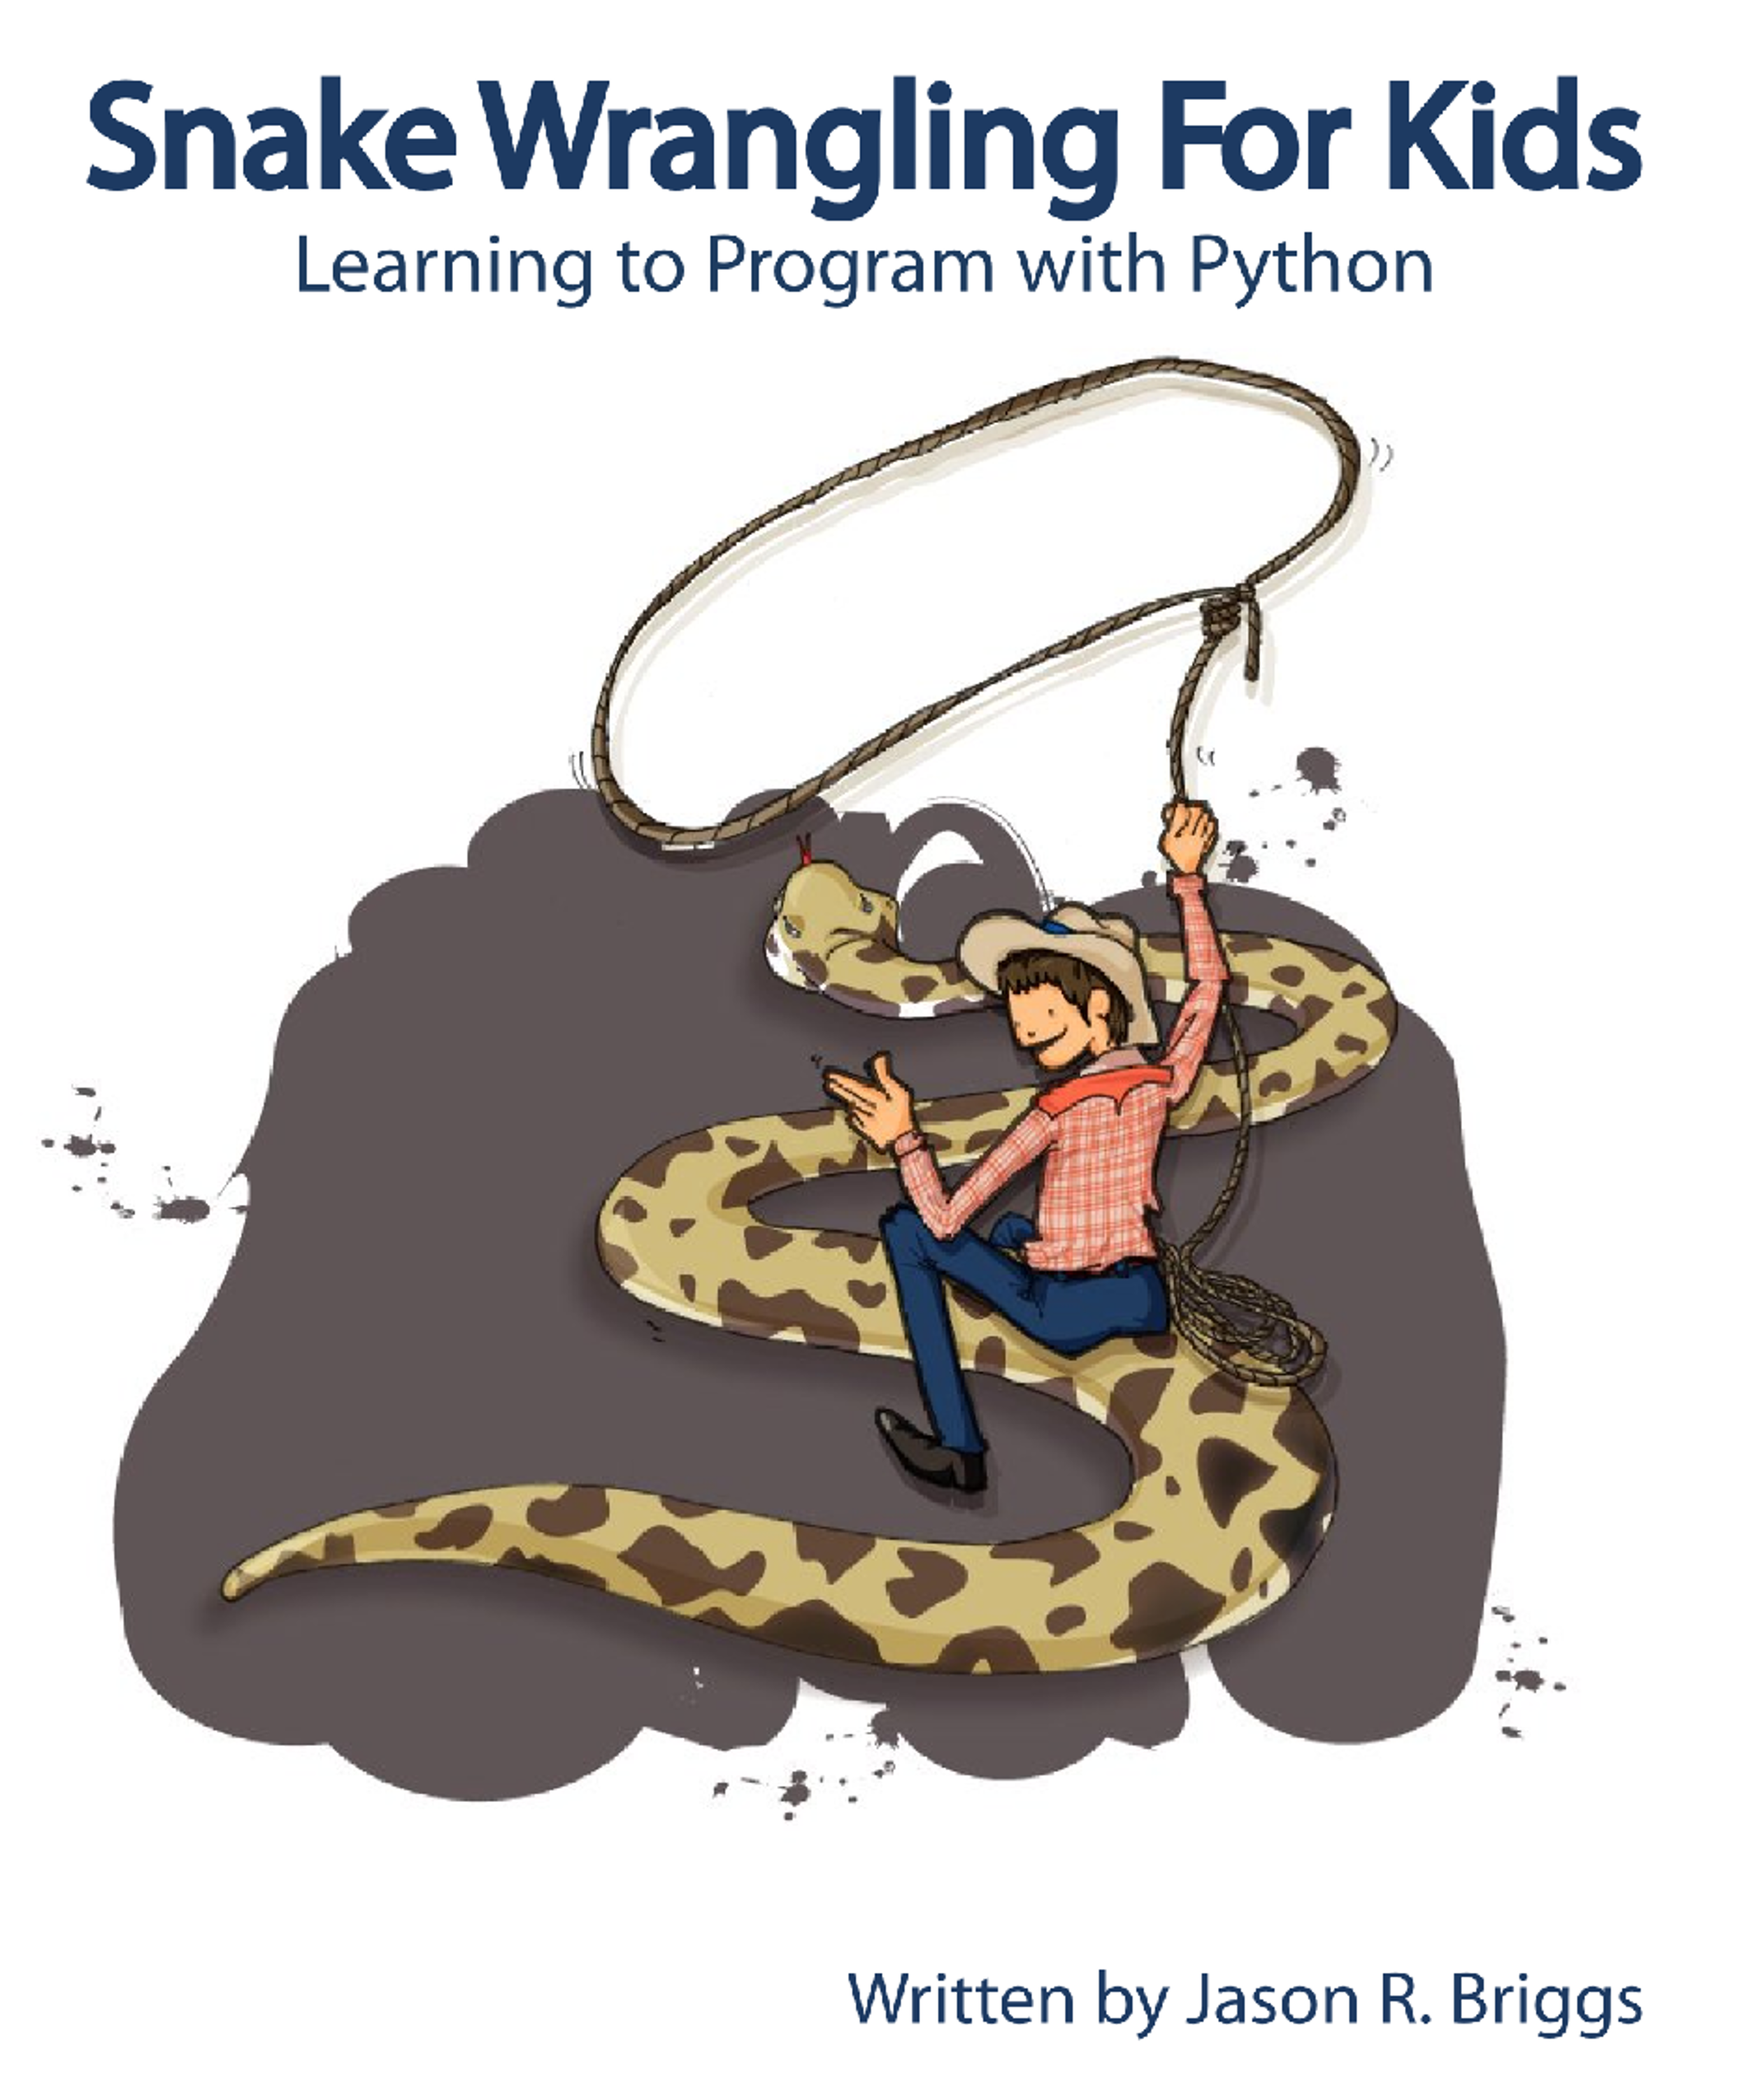
\includegraphics[width=0.9\paperwidth]{cover.eps}
\end{textblock*}
\begin{flushright}
\begin{WINDOWS}
\includegraphics[width=40mm]{windows-edition.eps} 
\end{WINDOWS}
\begin{MAC}
\includegraphics[width=40mm]{mac-edition.eps} 
\end{MAC}
\begin{LINUX}
\includegraphics[width=40mm]{linux-edition.eps} 
\end{LINUX}
\end{flushright}
\end{titlepage}
\end{FRONTCOVER}

\noindent
\textsf{\emph{Título original Snake Wrangling for Kids, Learning to Program with Python}}\\
por Jason R. Briggs\\
\\
Versión 0.7.7
\\\\
Copyright \copyright 2007.\\
\\
\textsf{\emph{Traducción al español: José Miguel González Aguilera}}\\
Versión 0.1.0\\
Copyright de la traducción \copyright 2009.\\
Website de la traducción: \href{http://code.google.com/p/swfk-es}{http://code.google.com/p/swfk-es}\\
\\
Publicado por... ah, en realidad... por nadie.\\
\\
Diseño de portada e ilustraciones realizado por Nuthapitol C.\\
\linebreak 
\noindent
Website:\\ \href{http://www.briggs.net.nz/log/writing/snake-wrangling-for-kids}{http://www.briggs.net.nz/log/writing/snake-wrangling-for-kids}\\ 

\noindent
Gracias a:\\
Guido van Rossum (por su benevolente dictadura del lenguaje Python), a los miembros de la lista de correo \href{http://www.python.org/community/sigs/current/edu-sig/}{Edu-Sig} (por sus útiles comentarios y consejos), al autor \href{http://www.davidbrin.com/}{David Brin} (el \href{http://www.salon.com/tech/feature/2006/09/14/basic/}{instigador} inicial de este libro), Michel Weinachter (por proporcionar unas versiones de mejor calidad de las ilustraciones), y a aquellas personas que aportaron información y erratas, incluidas: Paulo J. S. Silva, Tom Pohl, Janet Lathan, Martin Schimmels, and Mike Cariaso (entre otros).  Cualquiera que haya quedado fuera y no tuviera que quedar así, es debido a la prematura senilidad del autor.\\

\noindent
Licencia:\\
\\
\includegraphics[width=40mm]{by-nc-sa.eps}\\
Este trabajo está licenciado bajo la licencia de \emph{Reconocimiento-No comercial-Compartir bajo la misma licencia Creative Commons 3.0 España}. Para ver una copia de esta licencia, visita \href{http://creativecommons.org/licenses/by-nc-sa/3.0/es/}{http://creativecommons.org/licenses/by-nc-sa/3.0/es/} o envía una carta a Creative Commons, 171 Second Street, Suite 300, San Francisco, California, 94105, USA.\\

\noindent
A continuación se muestra un resumen de la licencia.\\

\noindent
Usted es libre de:
\begin{itemize}
 \item \textbf{Compartir} — copiar, distribuir y comunicar públicamente la obra 
 \item \textbf{Rehacer} — hacer obras derivadas
\end{itemize}
\noindent
Bajo las condiciones siguientes:
\begin{description}
 \item[Reconocimiento.] Debe reconocer los créditos de la obra de la manera especificada por el autor o el licenciador (pero no de una manera que sugiera que tiene su apoyo o apoyan el uso que hacer de su obra).
 \item[No comercial.] No puede utilizar esta obra para fines no comerciales.
 \item[Compartir bajo la misma licencia.] Si altera o transforma esta obra, o genera una obra derivada, sólo puede distribuir la obra generada bajo una licencia idéntica a ésta. 
\end{description}

\noindent
Al reutilizar o distribuir la obra, tiene que dejar bien claro los términos de la licencia de esta obra.\\

\noindent
Alguna de las condiciones puede no aplicarse si se obtiene el permiso del titular de los derechos de esta obra.\\

\noindent
Nada en esta licencia menoscaba o restringe los derechos morales del autor.\\

\vspace*{4cm}
\begin{center}
\includegraphics[width=5cm]{python-powered.eps}
\end{center}

\mainmatter

\pagestyle{plain}

\pagenumbering{roman}
\tableofcontents
